\begin{figure}[H]
  \centering
  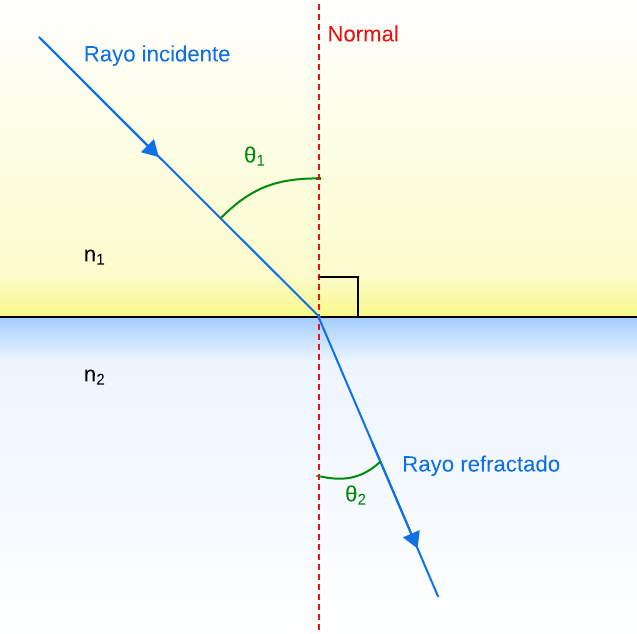
\includegraphics{imagenes/ley_snell.png}
  \caption{Ley de Snell}
\end{figure}

La formulación matemática es la siguiente:

\begin{listequbox}
  {n_1 \sin(\theta_1)=n_2 \sin(\theta_2)}{equleysnell}{Ley de Snell}
\end{listequbox}

Esta ley también es conocida como \textbf{Ley de refracción}.

Elementos:

\begin{itemize}
  \item \textbf{Rayo incidente:} Onda que viene de un primer medio y pasa a un segundo medio.
  \item \textbf{Rayo refractado:} Onda dentro de un segundo medio.
  \item \textbf{Normal:} Linea imaginaria perpendicular a la linea de separación entre ambos medios, en el punto donde el rayo incide.
  \item \textbf{Ángulo de incidencia $(\theta_1)$:} Ángulo formado entre el rayo incidente y la normal.
  \item \textbf{Ángulo de refracción $(\theta_2)$:} Ángulo formado entre el rayo refractado y la normal.
  \item \textbf{Índice de refracción 1 $(n_1)$:} Índice de refracción en el primer medio.
  \item \textbf{Índice de refracción 2 $(n_2)$:} Índice de refracción en el segundo medio.
\end{itemize}

El \textbf{índice de refracción}, representado por la letra $n$ minúscula, es una medida de como la luz se refracta al pasar de un medio a otro. Un índice más alto indica la onda viaja más lento, y en sentido contrario un índice más bajo indica que la onda viaja más rápido. Se calcula dividiendo la velocidad de la luz en el vacío $(c)$, ecuación \ref{equvelluz}, entre la velocidad de la luz en el nuevo medio $(v)$.

\begin{listequbox}
  {n = \dfrac{c}{v}}{equindrfr}{Índice de refracción}
\end{listequbox}

Al pasar de un primer medio con un índice $n_1$ a un segundo medio con un índice $n_2$, pueden ocurrir las siguientes situaciones:

\begin{itemize}
  \item \textbf{$n_1 = n_2$:} La velocidad en el segundo medio es igual. La onda se mueve sin alteraciones y no hay refracción.
  \item \textbf{$n_1 < n_2$:} La velocidad en el segundo medio es menor. La onda refractada se acerca a la normal.
  \item \textbf{$n_1 > n_2$:} La velocidad en el segundo medio es mayor. La onda refractada se aleja de la normal.
\end{itemize}

\begin{figure}[H]
  \centering
  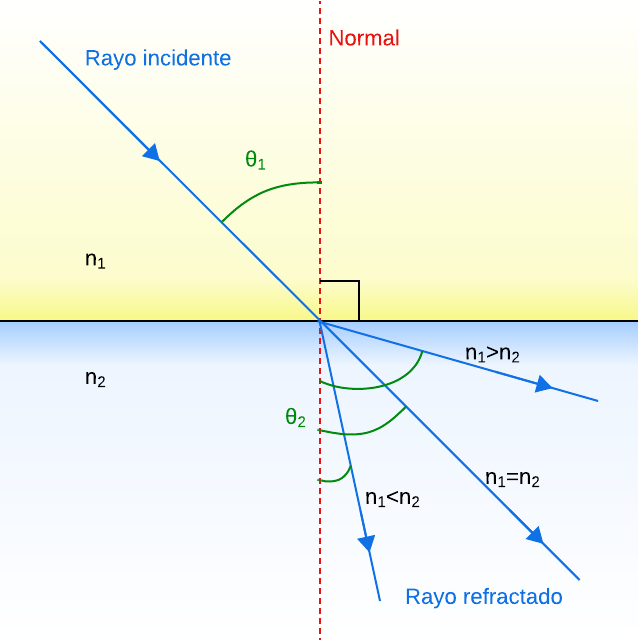
\includegraphics{imagenes/rayos_refractados.png}
  \caption{Índice de refracción y rayos refractados}
\end{figure}
